\section{Motivating example}
\begin{figure}[h]
\center{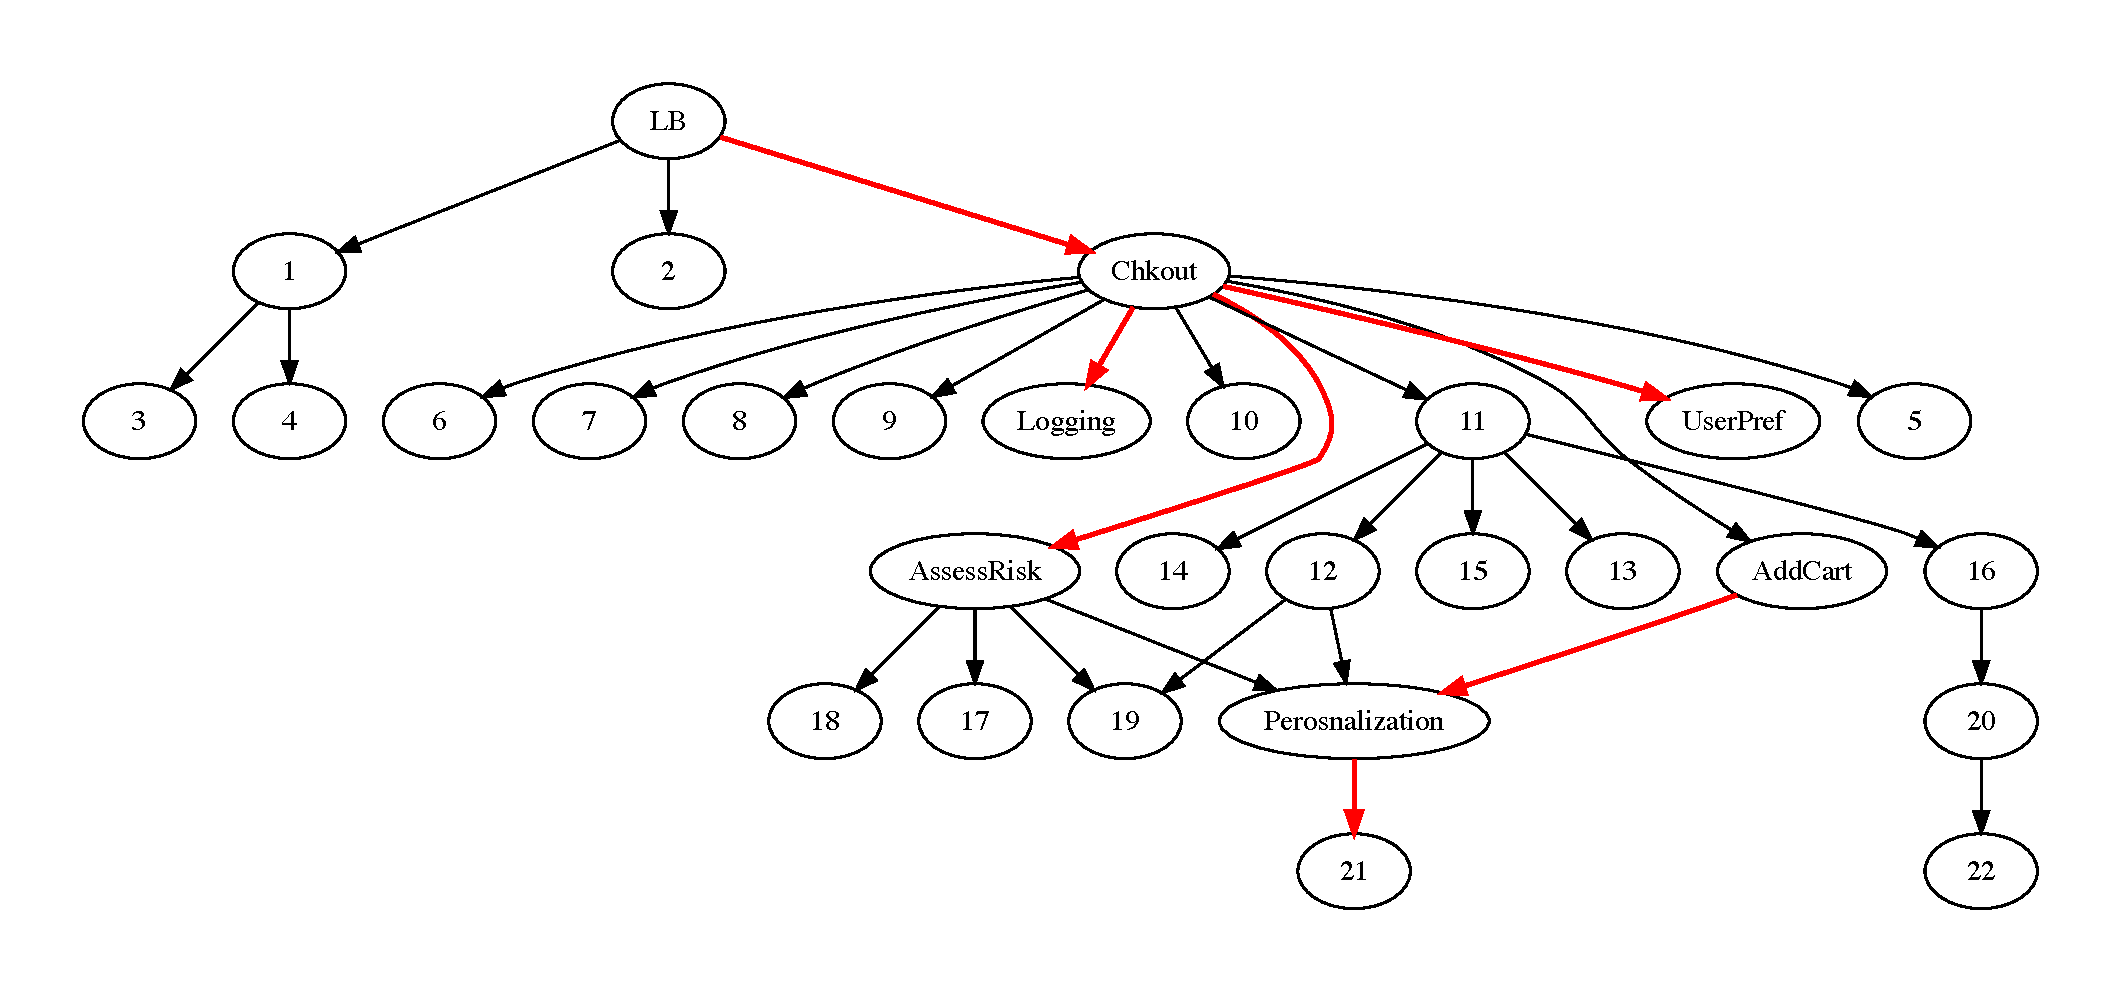
\includegraphics[scale=0.25]{anon_adrbk_fail.pdf}}
\caption{Example graph drawn from trace of an execution where the user was unable to checkout. The red lines indicate that the callee has returned an error to the caller}
\label{Failed_ex}
\end{figure}

To explain the triage process followed by site reliability engineers (SRE) when a failure occurs, consider the example of an user trying to buy items from an online store. 
%A successful checkout occurs when the user is able to place an order, else the checkout fails. 
During an outage, users might be unable to checkout. Figure~\ref{Failed_ex} shows the  call-graph of an user interaction involving checkout of items for a cart during an outage. The red lines in the graph indicate that the callee has returned an error to the caller. All services which return errors generate alerts. Of the services which are alerting, some of the alerts may be unrelated to the outage. Furthermore, if the crash of one or more services is related to the otuage, while all services from the root along the path leading to the crashed service(s) might be alerting,  the \textit{frontier} of failure is difficult to isolate.

When a system outage occurs, it is the job of a site reliability engineer (SRE) to find out why. Currently, the SRE sees a number of alerts, possibly from failures of RPC calls highlighted as red in the call graph, from the monitoring system.  Subsequently, based on the alerts, the SRE may consult aggregate data such as error rates and latency over sliding windows of time for services deemed problematic. The steps followed by an SRE while triaging an issue are as follows:
\begin{itemize}
\item Use domain knowledge about the dependencies between services to know which alerts are the result of transitive dependencies and must be ignored. \newline
As an example, the load balancer (LB) in the figure will be alerting as a result of its callee (Chkout) having returned an error message. This is indicated by the red line between LB and Chkout.  
An SRE with a good mental model of the system would conclude that since checkout (Chkout) has multiple downstream alerts, the alerts at LB are probably a result of the error being propagated up and try to dig deeper into one of the alerts from the downstream services. The reasoning is that a downstream service generating an alert is more likely to be a candidate for the proximal cause of the problem.  
\item Determine the proximal cause of outage\newline
Once a promising alert has been found, it is now time to look at the logs from the appropriate time to try to determine cause of failure. Determining the cause of the failure typically requires correlating events in multiple log files and the process can be both labor intensive and time-consuming. Based on the established cause, appropriate measures are then taken to mitigate failure which may include code, configuration or architectural changes.
\end{itemize}

By witnessing a large number of successful executions during steady state, we can learn models from steady state data such that we construct representations for traces which encode the structural properties of the underlying graphs corresponding to the traces. In the next section, we describe our technique for construction of trace embeddings and their use to provide hints for troubleshoot outages. 
%In the evaluation, we use clustering to demonstrate that embeddings outperform the state of the art, describe how we use simple distance measures on embeddings to address the problem described above and automatically generate hints about the proximal causes for the failure observed. 
%This is made possible by the fact that the embeddings encode information of structural neighborhoods.
%For outages which are not a result of service failures, a user entering invalid payment details perhaps or infrastructure failures, for example, appropriate next steps need to be taken. 